\section{Transition to the ``real world'' }\label{sec:rw_transition}
In order to investigate, how all the previous considerations about beamforming perform, when they are actually implemented, a series of measurements with a custom built speaker array has been conducted. A measurement protocol is given in \autoref{ax:directional_3}, as well as an overview over what individual measurements were conducted and what kinds of results were achieved. It is highly recommended to refer to the appendix when ambiguities occur while reading the following section.\\


\subsection{Ideal Approach}\label{ssec:ideal_approach}
If ressources allowed, the prefered method of testing the theoretical consideration regarding the array by doing a recursive approach. This means, that first, the speaker array is set up according to the expected position of the acoustic center from \autoref{sec:ac_center} and adjusted to be symmetrical and then the polar response from each of the speakers is measured seperately, similar to how it was done for \autoref{fig:05_11_single_main}. It has to be noted, that during measuring the individual polar responses, the membranes of the other loudspeakers should be fixed in order to achieve the most meaningful results. From these measurements, the actual position of the acoustic centers in relation to turning axis of the turntable can be derived similar to the approach that was proposed in \autoref{eq:ac_ctr} in \autoref{sec:ac_center}. Also, new correction tables for every individual speaker can be derived. The knowledge about the actual position of the acoustic centers with the array setup and the updated correction tables can then be used to run another optimization in order to generate updated \gls{sp}-parameters and filters. It is critical, that between measuring of the polar responses from the individual speakers and the measurment of the polar response from the array with beamforming enabled, the array is not taken down and put up again, as this would alter the positioning of the speakers with a probability bordering on certainty.
The measurement results from the polar response measurement of the speaker array would then be well suited to assess, how well the different array models (unaugmented analytical, augmented analytical, \gls{fdtd}-based) predict the actual behaviour of the array.

\begin{figure}[H]
\begin{subfigure}[c]{0.5\textwidth}
\includegraphics[width=0.85\textwidth]{05_11_A_pr.eps}
\subcaption{Speaker A, pressure}
\label{fig:05_11_A_pr_m}
\end{subfigure}
\begin{subfigure}[c]{0.5\textwidth}
\includegraphics[width=0.95\textwidth]{05_11_A_ph.eps}
\subcaption{Speaker A, phase}
\label{fig:05_11_A_ph_m}
\end{subfigure}\\
\hspace{0.1\textheight}
\begin{subfigure}[c]{0.5\textwidth}
\includegraphics[width=0.85\textwidth]{05_11_B_pr.eps}
\subcaption{Speaker B, pressure}
\label{fig:05_11_B_pr_m}
\end{subfigure}
\begin{subfigure}[c]{0.5\textwidth}
\includegraphics[width=0.95\textwidth]{05_11_B_ph.eps}
\subcaption{Speaker B, phase}
\label{fig:05_11_B_ph_m}
\end{subfigure}\\
\hspace{0.1\textheight}
\begin{subfigure}[c]{0.5\textwidth}
\includegraphics[width=0.85\textwidth]{05_11_C_pr.eps}
\subcaption{Speaker C, pressure}
\label{fig:05_11_C_pr_m}
\end{subfigure}
\begin{subfigure}[c]{0.5\textwidth}
\includegraphics[width=0.95\textwidth]{05_11_C_ph.eps}
\subcaption{Speaker C, phase}
\label{fig:05_11_C_ph_m}
\end{subfigure}\\
\caption{Polar responses of each speakers alone, final positioning, also found as \autoref{fig:05_11_single} in \autoref{ax:directional_3}}  
\label{fig:05_11_single_main}
\end{figure}

\subsection{The Actual Approach}\label{ssec:actual_approach}
Because of limited ressources, it was not possible to proceed as described in \autoref{ssec:actual_approach}. Instead, trial-and-error-based adjustments were made to the intital positioning of the loudspeakers. In order to do this, the array was set up based on the  expected position of the acoustic center from \autoref{sec:ac_center}. An initial measurement of the polar response was excecuted. The pressure characteristics are shown in \autoref{fig:05_11_initial_main}. Single adjustments were made to the positioning of the loudspeakers. After every adjustment, the polar response was measured and the results were compared to the inital measurement. The adjustments, that led to the polar response, that was declared final, suggest, that the acoustic centers of the loudspeakers are actual closer to the front edge of the speaker cabinets than the initial estimate of \SI{17}{\centi\meter}, that had been established in \autoref{sec:ac_center}. The rear speaker \texttt{A} has been moved towards the front by \SI{4.5}{\centi\meter} from its intial position. The side speakers have been moved towards the inside by \SI{2}{\centi\meter} each, and their azimuth angle has been increased to approx. \SI{55}{\degree}. \autoref{fig:05_11_final_main} shows the polar response, that has been measured with the final positiong. It is apparent, that, compared to the initial measurement, the attenuation of the backlobe has been increased.

\begin{figure}[H]
\begin{subfigure}[c]{0.5\textwidth}
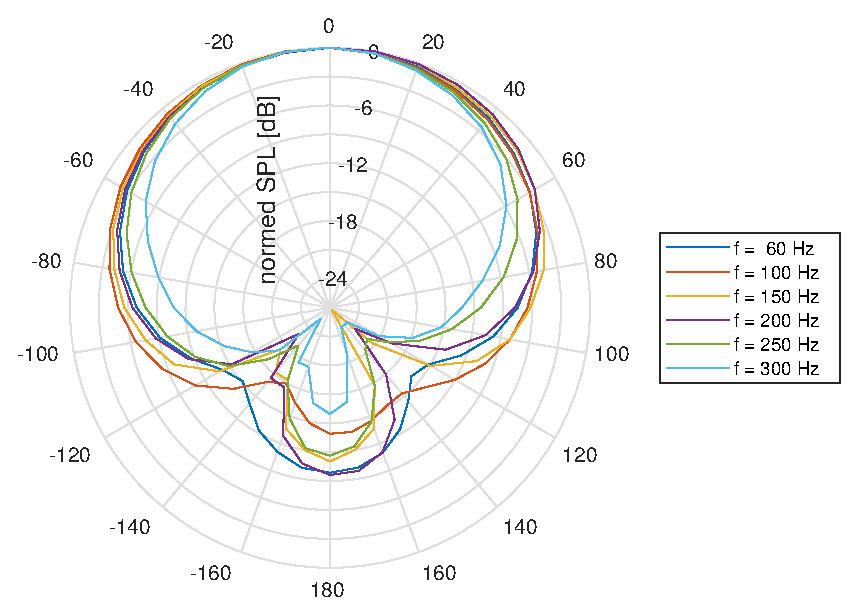
\includegraphics[width=0.95\textwidth]{05_11_initial_pr.eps}
\subcaption{Pressure characteristics, initial positioning, vgl. \autoref{fig:05_11_initial}}
\label{fig:05_11_initial_main}
\end{subfigure}
\begin{subfigure}[c]{0.5\textwidth}
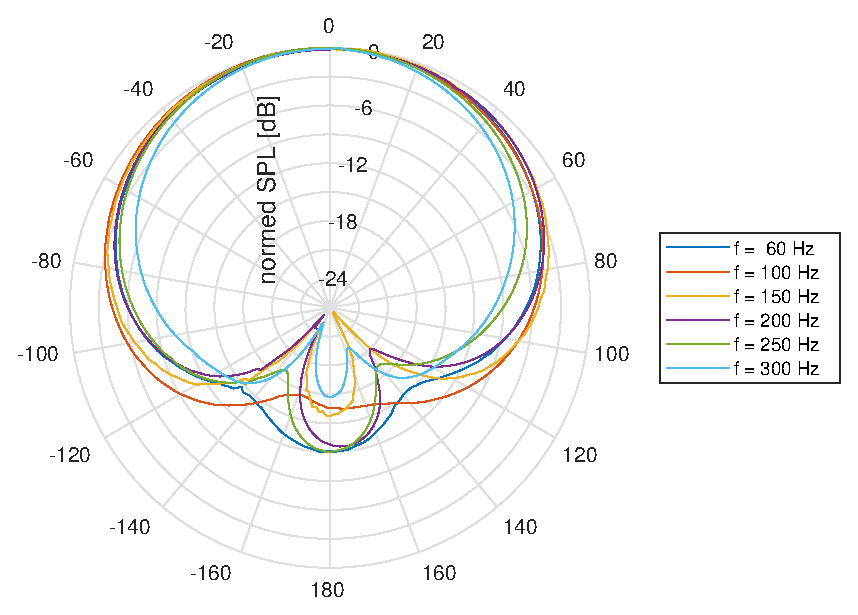
\includegraphics[width=0.95\textwidth]{05_11_final_pr.eps}
\subcaption{Pressure characteristics, final positioning, vgl. \autoref{fig:05_11_final}}
\label{fig:05_11_final_main}
\end{subfigure}\\
\caption{Polar plot, initial vs. final positioning, the initial polar response has been measured with lower angular resolution than the final one.}  
\label{fig:05_11_adjustments}
\end{figure}